\documentclass[12pt]{article}
%--------------------   start of the 'preamble'
%
\usepackage{graphicx,amssymb,amstext,amsmath,color}
\usepackage[margin=2cm]{geometry}
\usepackage{abstract}
\usepackage{setspace}
\usepackage[footnotesize,bf]{caption}

% TABLE
\usepackage{multicol,hhline,colortbl,multirow}
\usepackage{braket}
\usepackage{siunitx}
\usepackage{hyperref}
\usepackage{authblk}
\usepackage{siunitx}
\usepackage{mathrsfs}
%%\usepackage[sort&compress]{natbib}
%%\bibpunct{(}{)}{,}{a}{, }{;}
%
\usepackage[sort&compress]{natbib}
\bibpunct{[}{]}{,}{s}{}{;}


\definecolor{gray}{gray}{0.8}
\def\mobunits{\square\centi\meter\per\volt\per\second}
\def\gcm{\gram\per\cubic\centi\meter}
\def\ccg{\cellcolor{gray}}

\renewcommand{\labelitemii}{$\circ$}
\renewcommand{\bibname}{References}


\title{MorphCT Results - Simple Crystal System}
\author{Matthew Jones}
\date{\today}

\begin{document}
\maketitle


\section{Crystal Test System}


\subsection{Device Morphology}

\begin{figure}[h!]\centering
	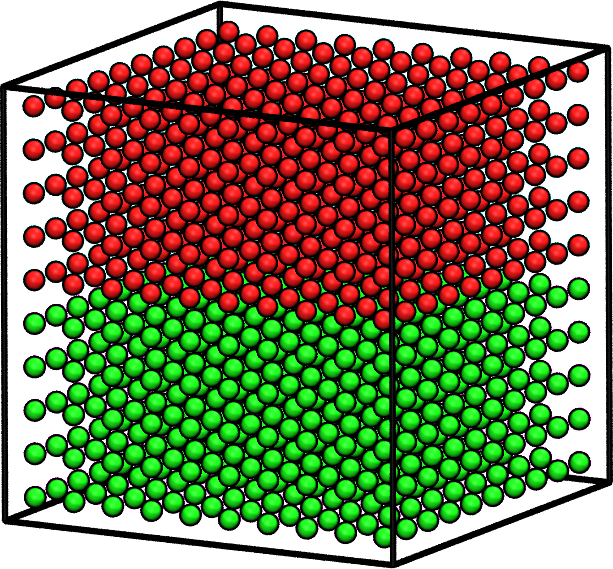
\includegraphics[width=0.3\textwidth]{Figures/device.png}
    \caption{The test simulation used. Red `atoms' are donor, green `atoms' are acceptor.}
	\label{fig:device}
\end{figure}



\subsection{Parameters}

Each `atom' in the cell is connected to its Voronoi neighbour using a TI $= 0.1 eV$.
Charge carriers are permitted to hop across the periodic boundaries at the top and bottom of the cube in order to be extracted at the anode and cathode respectively.

The device parameters were based on experimentally realistic values for P3HT:PCBM devices.
\textcolor{red}{Add a table of parameters here.}


\subsection{Results}


\begin{figure}[h!]\centering
	\begin{tabular}{cc}
		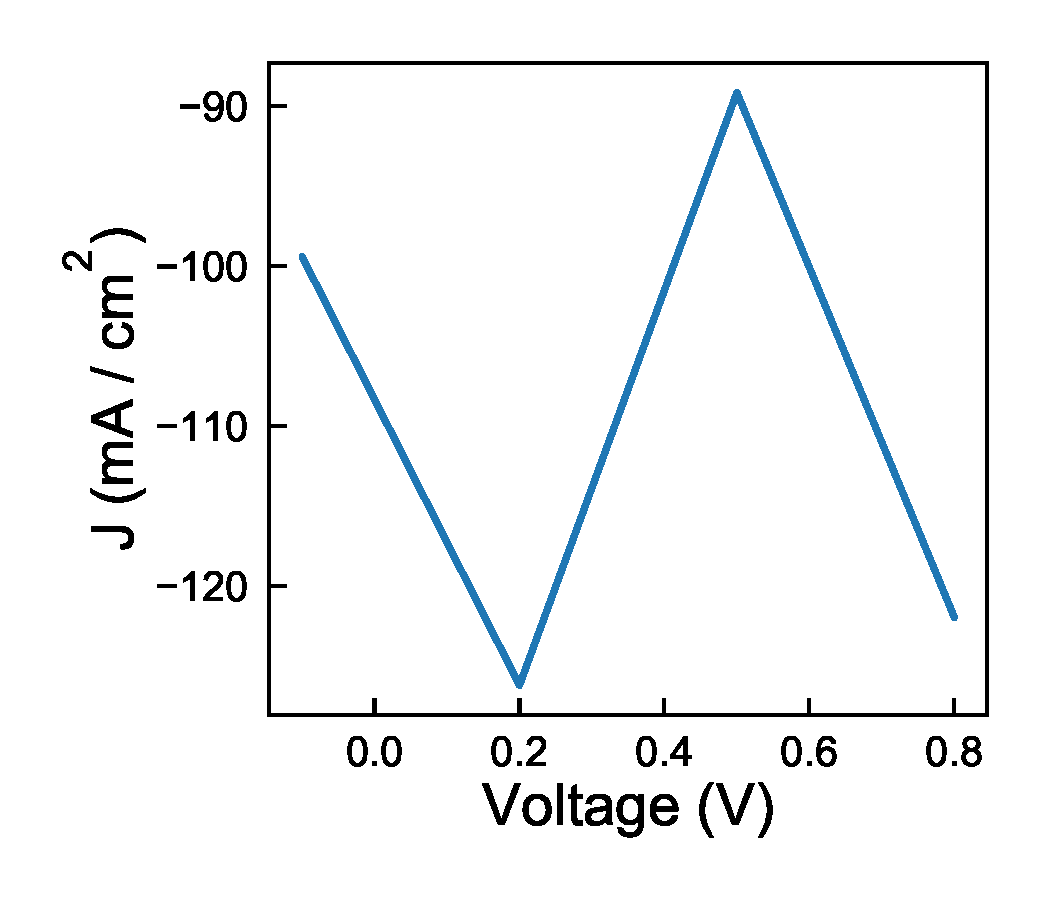
\includegraphics[width=0.5\textwidth]{Figures/firstJV.pdf}&
		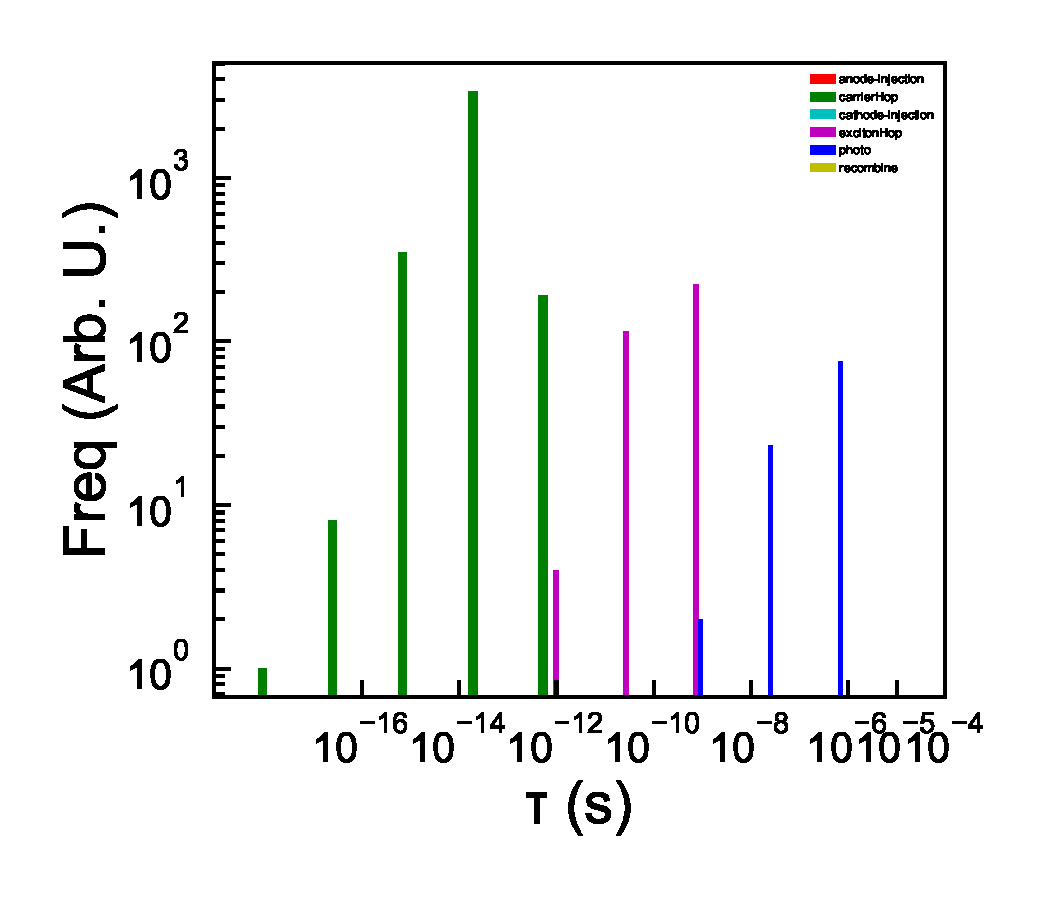
\includegraphics[width=0.5\textwidth]{Figures/firstEventTime.pdf}\\
	\end{tabular}
    \caption{The J-V curve from the device, and the corresponding event time distribution when the input parameters were based on realistic values from experiment.}
	\label{fig:device1}
\end{figure}


Note that the JV curve looks pretty horrible. 
The absolute values of $\sim$ 100 mA/cm$^{2}$ are exactly in line with the expected output from a P3HT/PCBM device, suggesting that the \textcolor{blue}{arbitrary tunable parameters} we use to slow down exciton hopping to get the expected diffusion lengths, and photoinjection restriction parameters are about right.
Effectively, there is no voltage dependence, as the current is constant across the full sweep.
The reason for this becomes clear when examining the event time distribution.
Photoinjections occur several (~10) orders of magnitude more slowly in time than the carrier hops.
Considering a charge carrier heading directly for the contact would only need 5 hops to reach the contact from the point of dissociation, this means that the device is always empty by the time the next photoinjection comes along.
In the absence of charge carriers in the system, the extracted photocurrent is therefore solely limited by the photoinjection rate, washing out the voltage trend.


In order to prevent this, the photoinjection rate must be increased to bring it in line with the carrier hopping.


\subsection{Increased photoinjection rate}


\textcolor{red}{New parameters here}

\begin{figure}[h!]\centering
	\begin{tabular}{cc}
		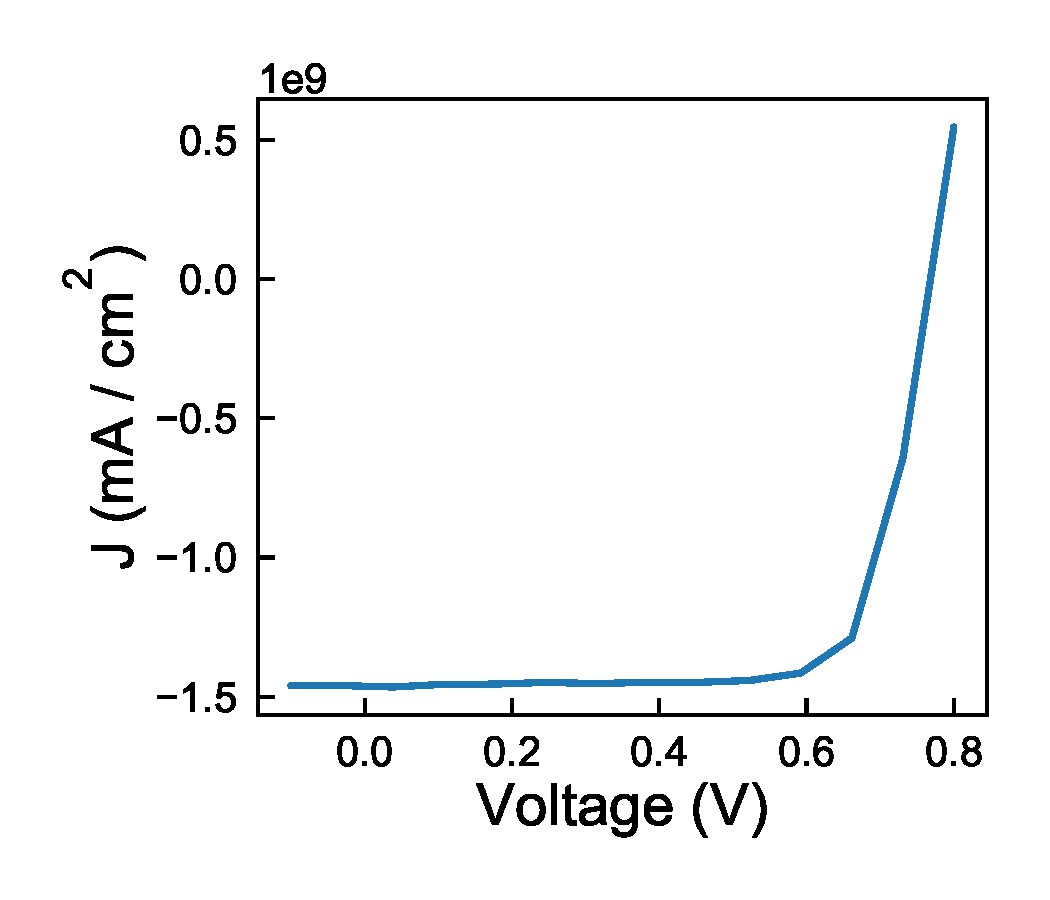
\includegraphics[width=0.5\textwidth]{Figures/secondJV.pdf}&
		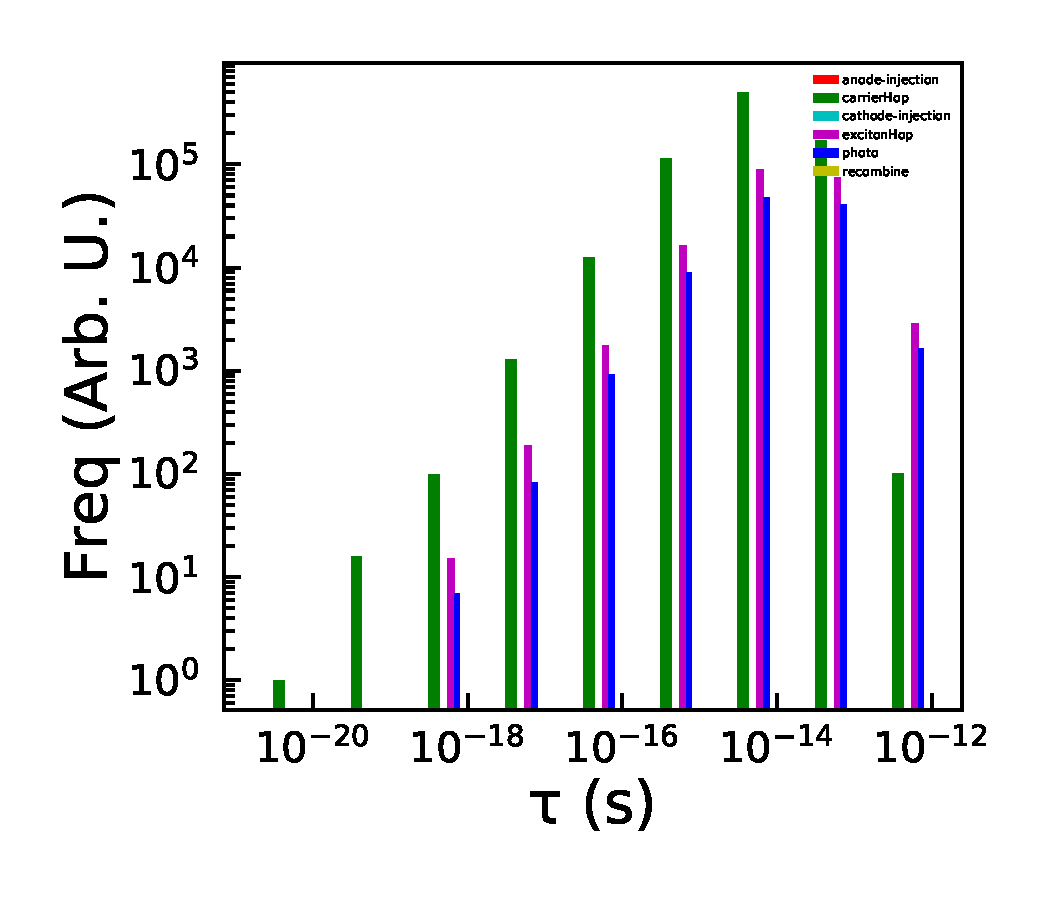
\includegraphics[width=0.5\textwidth]{Figures/secondEventTime.pdf}\\
	\end{tabular}
    \caption{The J-V curve from the device, and the corresponding event time distribution when the input parameters were tweaked to get good event time distribution curves.}
	\label{fig:device2}
\end{figure}


Note that increasing the photoinjection rate, and aligning the photoinjection rates with the hopping rates has dramatically improved the J-V trend.
This also indicates that the field calculations and coulombic effects in the device are being calculated correctly, otherwise there would be no J-V curve.
Note that dark current injection has been removed here, as it can cause issues with carrier extraction because the device itself is so small.


This marks the end of the usefulness of this crystal test.
We need a proper network with realistic parameters so that we can tune our simulations to get useful results.
These 10nm donor, acceptor and mixed, networks with realistic experimental densities are currently being obtained by OPV\_CG and MorphCT, and their data can be reported soon.

\bibliography{refs}
\bibliographystyle{unsrt}


\end{document}
